\newpage
\subsection{Krzyżowanie}

Krzyżowanie jest podstawowym mechanizmem tworzenia potomstwa na podstawie wartości przyjmowanych przez rodziców. W stworzonej implementacji pobierana jest połowa wartości od każdego z nich, a ich suma stanowi nowego potomka

\subsubsection{Kod źródłowy}

\begin{lstlisting}[linewidth=16.0cm]
myCrossover <- function (ga_object, parents)
{
  # Pobranie rodzicow do skrzyzowania
  # i zainicjalizowanie nimi potomstwa
  parents <- ga_object@population[parents,,drop = FALSE]
  parCol <- ncol(parents)
  parRow <- nrow(parents)
  children <- parents

  
  for (i in 1:parCol)
  { 
	for(j in 1:parRow)
	{
	  if (j == parCol) {  
	    nextCol <- 1 
	  }
	  else {
	    nextCol <- j+1
      }
      
      # Resultat krzyzowania - 
      # suma 1/2 wartosci kazdego rodzica z wybranych pol
	  newChild <- parents[i, j]/2 + parents[i, nextCol]/2
	  children[i, j] <- newChild
	}
  }

  out <- list(children = children, fitness = rep(NA,2))
  return(out)
}
\end{lstlisting}

\subsubsection{Wyniki badań}

\begin{figure}[H]
	\centering
	\hspace*{-0.8in}
	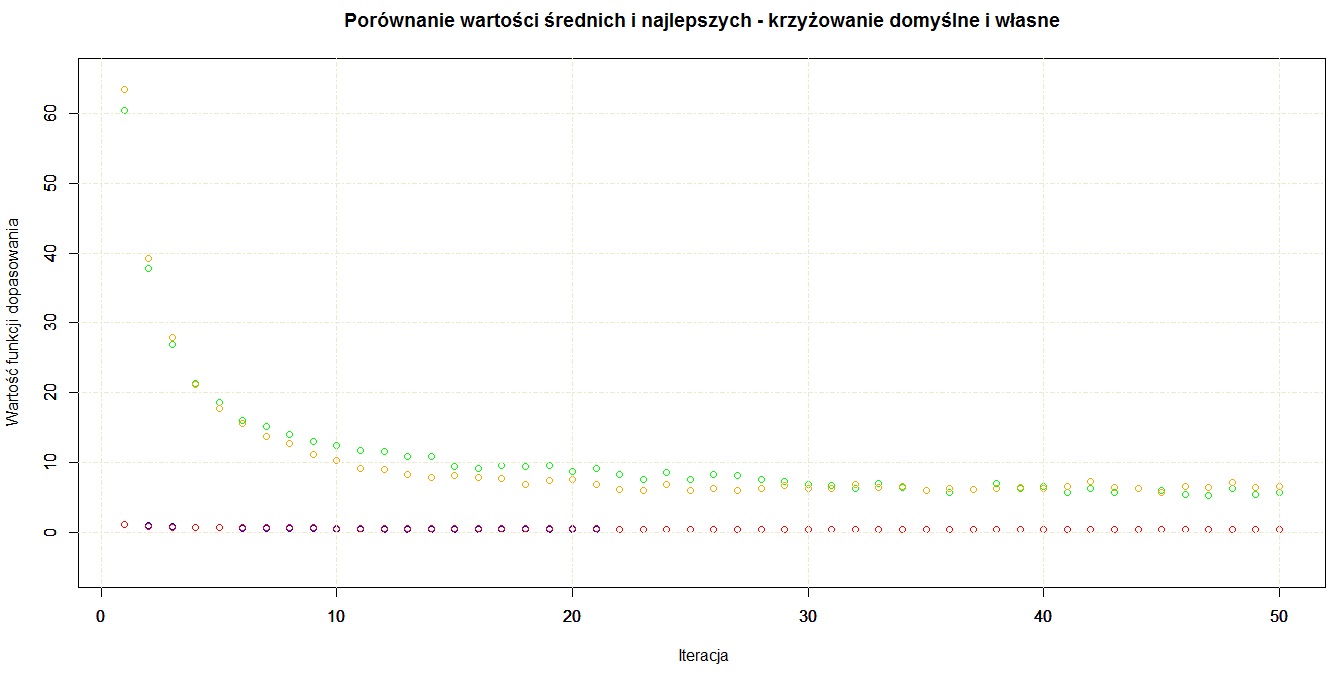
\includegraphics[scale = 0.5]{img/zad1/cross_0_2}
	\caption{Wykres dla prawdopodobieństwa krzyżowania 0.2}  
	\label{rys:cross_0_2} 
\end{figure}


\begin{figure}[H]
	\centering
	\hspace*{-0.8in}
	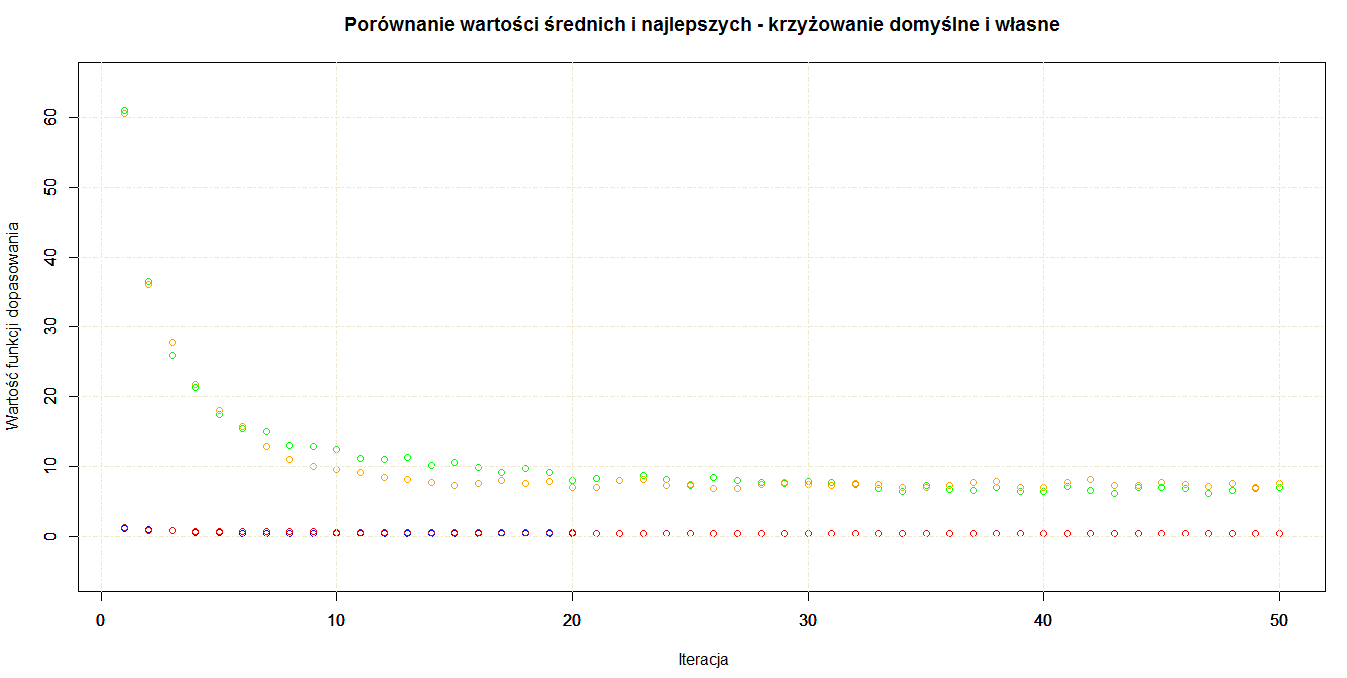
\includegraphics[scale = 0.5]{img/zad1/cross_0_5}
	\caption{Wykres dla prawdopodobieństwa krzyżowania 0.5}  
	\label{rys:cross_0_5} 
\end{figure}


\begin{figure}[H]
	\centering
	\hspace*{-0.8in}
	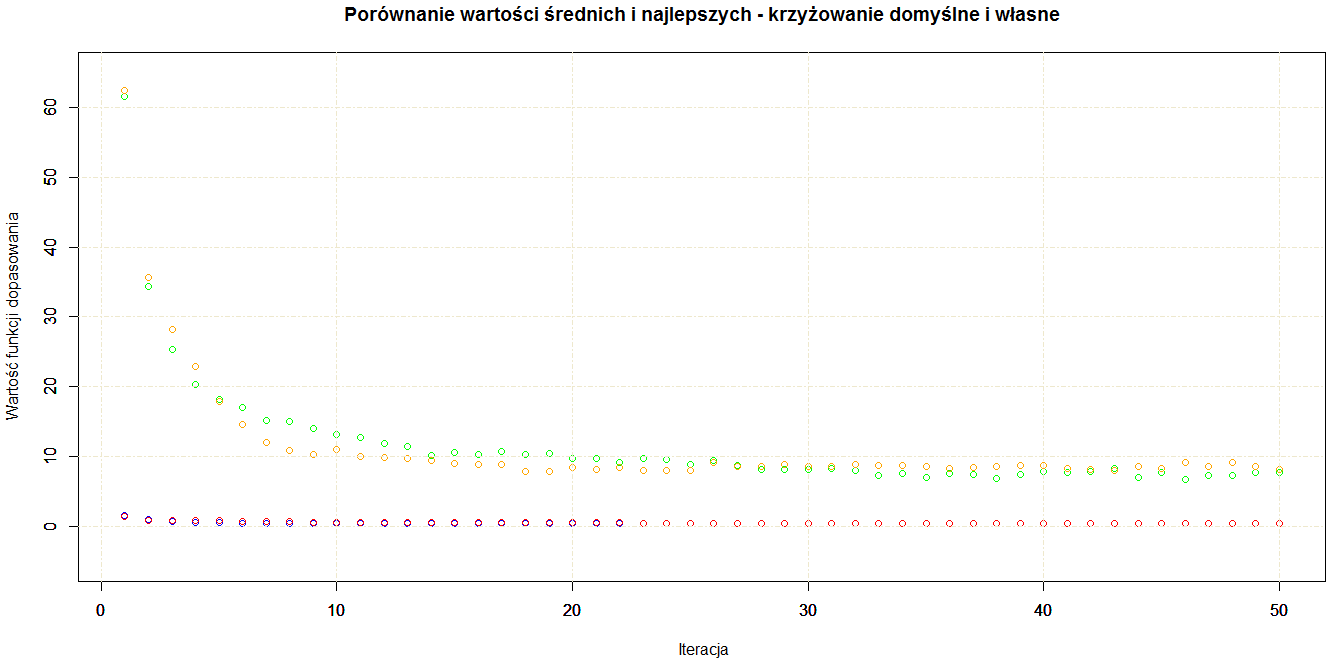
\includegraphics[scale = 0.5]{img/zad1/cross_0_7}
	\caption{Wykres dla prawdopodobieństwa krzyżowania 0.7}  
	\label{rys:cross_0_7} 
\end{figure}


\begin{figure}[H]
	\centering
	\hspace*{-0.8in}
	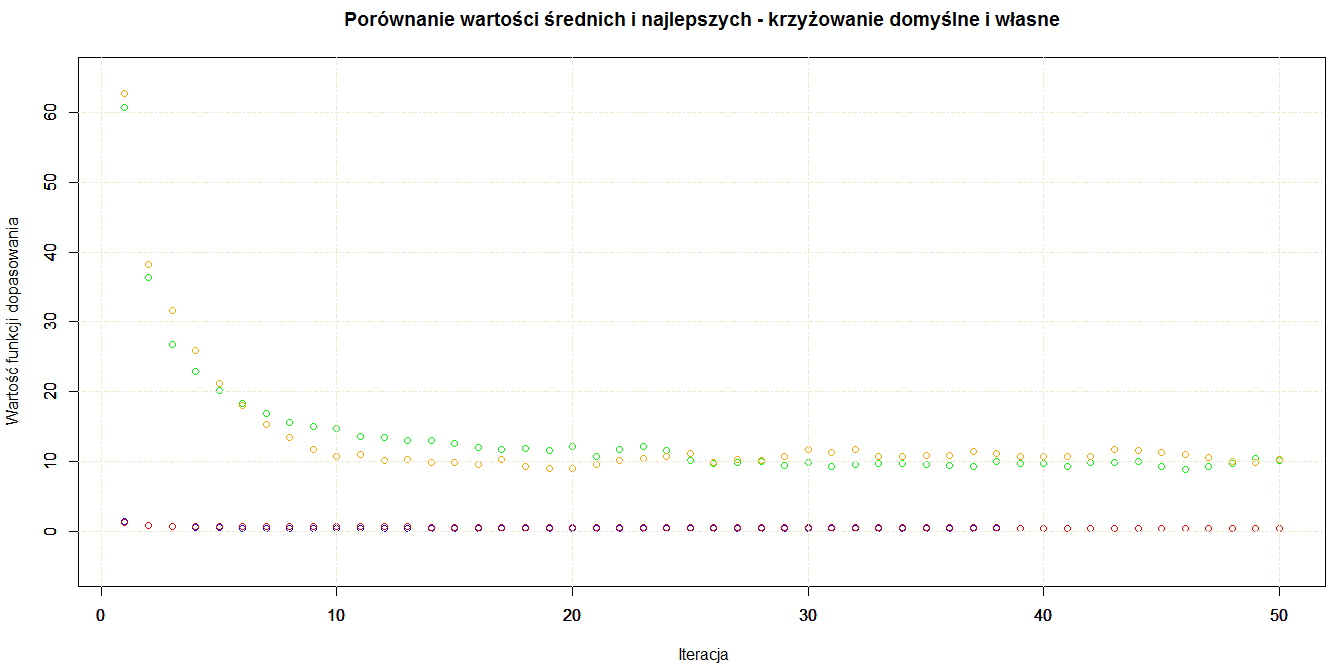
\includegraphics[scale = 0.5]{img/zad1/cross_1}
	\caption{Wykres dla prawdopodobieństwa krzyżowania 1}  
	\label{rys:cross_1} 
\end{figure}

\vline

\subsubsection{Wnioski}

\begin{table}[!h]
	\centering
	\caption{Wartości średnie i najlepsze osobnika dla domyślnej i własnej funkcji krzyżowania}
	\label{cross_porownanie}
	\hspace*{-0.5in}
	\begin{tabular}{|c|c|c|c|c|}
		\hline
		\textbf{Prawdopodobieństwo} & \multicolumn{2}{c}{\textbf{Krzyżowanie domyślne}}  & \multicolumn{2}{|c|}{\textbf{Krzyżowanie własne}} \\ \cline{2-5}
		\textbf{krzyżowania} & Wartość średnia & Najlepszy wynik & Wartość średnia & Najlepszy wynik \\ \hline
		
		0.2 & 5.697605 & 0.399347 & 6.538159 & 0.440933 \\
		0.5 & 6.973119 & \textbf{{\color{green} 0.398064 }} & 7.590295 & 0.457468 \\
		0.7 & 7.753576 & 0.398096 & 8.148286 & 0.464140 \\
		1   & 10.206810 & 0.398485 & 10.375570 & 0.476180  \\ \hline      
	\end{tabular}
\end{table}

Tak jak w przypadku mutacji, krzyżowanie nie wpłynęło na poprawę najlepszego wyniku, wręcz przeciwnie - zwiększanie prawdopodobieństwa krzyżowania coraz bardziej pogarszało otrzymywane wartości. Rezultat najbardziej zbliżony do minimum globalnego został uzyskany dla parametrów domyślnych i wbudowanych funkcji.\\
Średnie populacji dla tych dwóch różnych implementacji przeplatały się, oscylując wokół zbliżonych wartości.